\paragraph{1. Library toevoegen}
Om de navigatie en het laadscherm te kunnen gebruiken moeten de juiste libraries aan 
de root van het project worden toegevoegd. Deze worden toegevoegd met volgende commandos:
\begin{minted}{bash}
npm install @react-navigation/native
npm install react-native-screens
npm install react-native-safe-area-context
npm install @react-navigation/bottom-tabs
\end{minted}

\paragraph{2. onCreate methode toevoegen}
Om de navigatie te gebruiken moeten een \textbf{onCreate} methode worden toegevoegd aan het
\textit{android/app/src/main/java/com/project/MainActivity.java} bestand.
\begin{minted}{java}
import android.os.Bundle;
// ...
public class MainActivity extends ReactActivity {
  // ...
  @Override
  protected void onCreate(Bundle savedInstanceState) {
    super.onCreate(null);
  }
  // ...
}
\end{minted}

\paragraph{3. Dependencies toevoegen}
Om het laadscherm te gebruiken moeten de juiste dependencies worden toegevoegd aan het
\textit{android/app/build.gradle} bestand.
\begin{minted}{java}
dependencies {
  // Andere dependencies
  implementation("androidx.core:core-splashscreen:1.0.0")
}
\end{minted}

\paragraph{4. Laadscherm toevoegen}
Om een eerste laadscherm te genereren kan volgend commando worden gebruikt:
\begin{minted}{bash}
npx react-native generate-bootsplash path/to/icon.png
    --background-color "#000000" 
    --logo-width=100 
    --assets-path=assets 
    --flavor=main 
    --platforms=android,ios
\end{minted}
Daarna moet er een stijl worden aangemaakt om het laadschem te tonen. Dit gebeurt in 
het \textit{android/app/src/main/res/values/styles.xml} bestand.
\begin{minted}{xml}
<style name="BootTheme" parent="Theme.SplashScreen">
    <item name="windowSplashScreenBackground">@color/bootsplash_background</item>
    <item name="windowSplashScreenAnimatedIcon">@mipmap/bootsplash_logo</item>
    <item name="postSplashScreenTheme">@style/AppTheme</item>
</style>
\end{minted}
Om dan bij het opstarten van de applicatie het laadscherm eerst te tonen moet de volgende 
lijn in het \textit{android/app/src/main/AndroidManifest.xml} bestand worden aangepast.
\begin{minted}{xml}
<application
  android:name=".MainApplication"
  android:label="@string/app_name"
  android:icon="@mipmap/ic_launcher"
  android:roundIcon="@mipmap/ic_launcher_round"
  android:allowBackup="false"
  android:theme="@style/BootTheme"> <!-- Verander deze lijn -->
  <!-- ... -->
</application>
\end{minted}
Tot slot kan het laadscherm geïnitaliseerd worden door volgende regels toe te voegen aan het
\textit{android/app/src/main/java/com/project/MainApplication.java} bestand.
\begin{minted}{java}
import com.zoontek.rnbootsplash.RNBootSplash;

public class MainApplication extends Application implements ReactApplication {
  // ...
  @Override
  public void onCreate(Bundle savedInstanceState) {
    RNBootSplash.init(this); // Voeg deze lijn toe
    super.onCreate(savedInstanceState);
  }
  // ...
}
\end{minted}

\paragraph{5. Navigatie toevoegen}
Om de navigatie te gebruiken moeten alle componenten in een 
\textbf{NavigationContainer} component worden gestoken. Dit wordt gedaan door volgende regels toe te voegen
aan het \textit{App.tsx} bestand:
\begin{minted}{javascript}
import { NavigationContainer } from '@react-navigation/native';

export default function App() {
  return (
    <NavigationContainer>
      {/* ... */}
    </NavigationContainer>
  );
}
\end{minted}

\paragraph{6. Bottom Tab navigatie toevoegen}
Om de bottom tab navigatie te gebruiken moet een \textbf{createBottomTabNavigator}
functie worden aangemaakt. Dit wordt gedaan door de volgende regels toe te voegen aan het \textit{App.tsx} bestand:
\begin{minted}{javascript}
import { createBottomTabNavigator } from '@react-navigation/bottom-tabs';

const Tab = createBottomTabNavigator();

export default function App() {
  return (
    <NavigationContainer>
      <Tab.Navigator>
        {/* ... */}
      </Tab.Navigator>
    </NavigationContainer>
  );
}
\end{minted}
Daarna kunnen de verschillende schermen worden toegevoegd aan de \textbf{Tab.Navigator} component.
\begin{minted}{javascript}
<Tab.Navigator>
    <Tab.Screen name="Home" component={HomeScreen} />
    <Tab.Screen name="Second" component={SecondScreen} />
    <Tab.Screen name="Third" component={ThirdScreen} />
</Tab.Navigator>
\end{minted}

\paragraph{7. Applicatie maken}
Met deze informatie wordt een applicatie met een laadscherm aangemaakt.
Het laadscherm zal verdwijnen vanaf de 
applicatie gerenderd is. Daarna is er een bottom tab navigatie dat navigeert tussen 
de drie verschillende schermen. 
\begin{figure}[H]
    \centering
    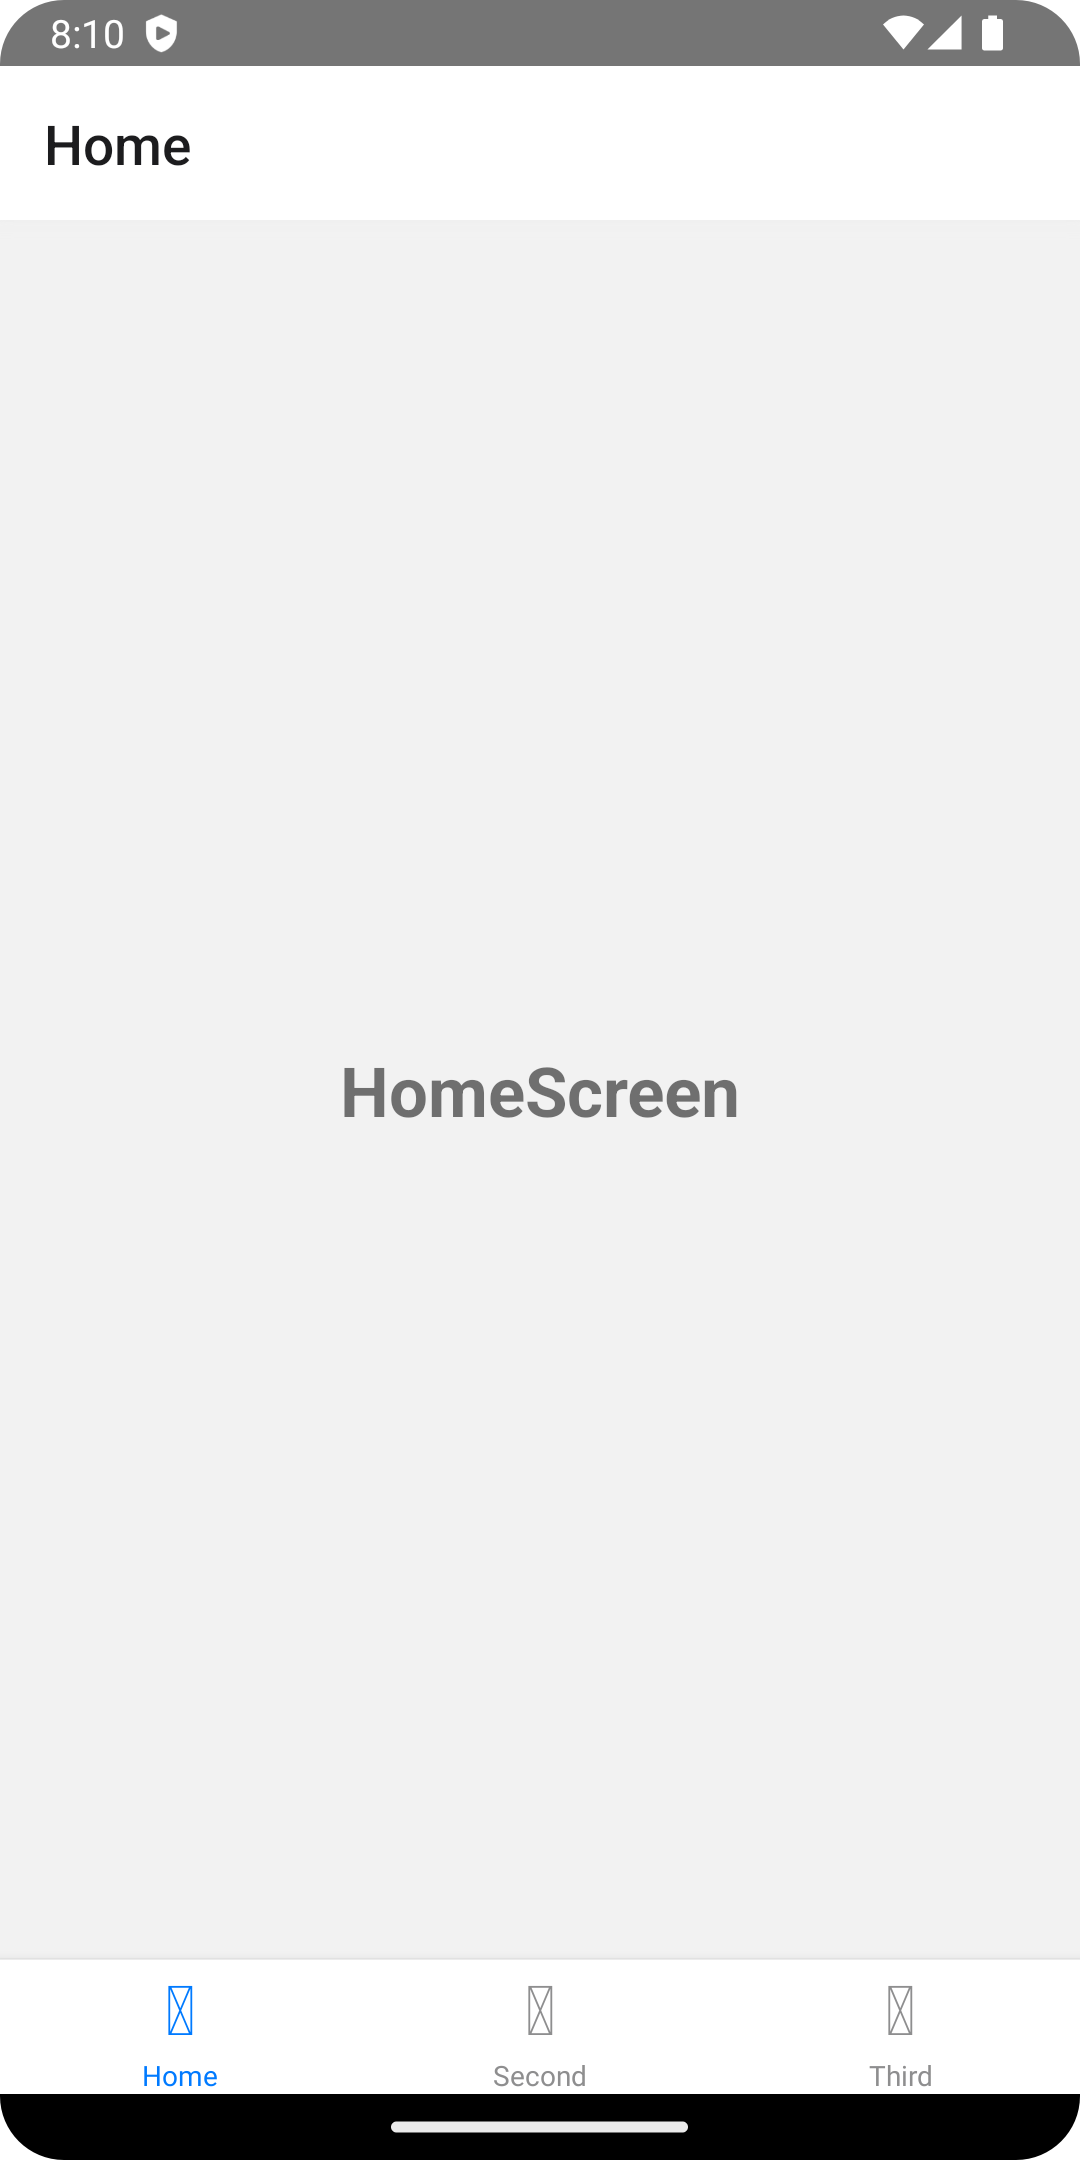
\includegraphics[height=0.4\textheight]{basis_layoutcross.png}
    \caption{Layout van applicatie voor de basisfunctionaliteiten bij React Native.}
\end{figure}
